\chapter{Uncovering online tapestries: Ecological patterns in information ecosystems}\label{chp:4}

Many complex systems, such as ecosystems or social systems, can benefit from interdisciplinary approaches to be better understood and effectively managed. In particular, online communication systems are composed of many interconnected agents, and fully characterizing  them  requires developing innovative models that draw from insights from multiple fields. As a case in point, in Chapter~\ref{chp:3}, we proposed a driver for collective attention --the optimization of visibility-- and validate it using an ecology-inspired model. In this Chapter, we investigate the dynamics of online social networks at an alternative scale, which looks at the fingerprints of drivers and constraints in a more general way. They are not obvious a priori, and to infer such characteristics we look for quantitative invariants that are consistently repeated, patterns. Following the bridge we drew in this thesis between natural and information ecosystems, we assume that ecological and social complex systems, despite the differences in the nature of their microscopic description, may exhibit similar complex behavior in the form of patterns on the macroscopic scale. Identifying a pattern is the first step to discovering the  drivers of the dynamics, as every proposed process must be able to reproduce those patterns.\\
   
%%%%%%%%%%%%%%%%%%%%%%%%%%%%%%%%%%%%%%%%%%%%%%%%%%%%%%%%%%%%%%%%%%%%%%%%%%%%%%%%%%%%%%%%%%%%%%%%%%%%
\section{Why: the purpose of looking and finding patterns\label{chp:4:1}}

Here, we ask whether information ecosystems share the same general laws found in natural ecosystems. Given the analogies that can be drawn between the two systems and their success in creating new insight and applications \cite{borge2017emergence,palazzi2021ecological,plata2021neutral,calleja2021quantifying,tovo2021upscaling}, this research question is the logical step towards a fruitful cross-fertilization of the two worlds. If hashtags are seen as species, we can start keeping track of what we observe in online social systems to analyze what is happening with an ecological lens. By counting individuals in ecosystems, we have discovered several universal laws; such as that in any community of species, there are a few very abundant species and many rare species --the so-called Relative Species abundance distribution 
\cite{brown1995macroecology,preston1948commonness}. Does the social counterpart of this pattern exist? If so, would it have the same shape and features as the natural version? For example, would a potential abundance distribution of hashtags change with the size of the system as the species' abundances change with the scale of the community? \\

The possible existence of common patterns would suggest that there may be universal principles that drive the dynamics of natural ecosystems and online social networks (information ecosystems). Then, all the new questions that arise from this ecologically-inspired approach could take advantage of the theory once developed to explain the patterns in nature, for example, niche theory \cite{hutchinson1957concluding} and neutral dynamics \cite{hubbell2001unified} (that it was in turn borrowed from molecular genetics \cite{kimura1983neutral}). Another benefit of finding general patterns is that they have allowed for some simplification that has exceptional predictive power. In ecology, they are used to estimate the number of species that will become extinct as a result of habitat destruction, and how many species are present in ecosystems that are too large or difficult to sample extensively \cite{brown1995macroecology}. Recently, this extrapolation approach has been applied in human activity data to upscale the number of components in human communications (emails, words) as the size of the system increases \cite{tovo2021upscaling}. \\

In this context, we look for emerging patterns among a very heterogeneous group of datasets. They are reasonably not expected to share the same type of constraints, selection criteria, or optimization principles, given the radically different nature of their discussions and sampling methods \cite{zubiaga2018}. In turn, the selected patterns are widely known in ecology and revolve around complementary aspects of communities like their fluctuations in time and scale. 
%If these quantitative patterns are found in all our datasets, they may provide information about the commonalities of information ecosystems. 
 We then take a step further and investigate some aspects of the possible origin of the patterns, resampling our datasets according to a null model to answer how much of the observed patterns may be due to chance. In particular, we use a multinomial sampling model that only takes the frequencies of the hashtags into account. It lacks the details and constraints of the environment in which the hashtags have been generated, making it a useful null model that has been tested in the study of microbial communities \cite{grilli2020macroecological} or component systems like Lego sets \cite{lego}.
 
%- In many, but not all, of these models a preferential attachment principle is at the origin of the emergence of the power-law distribution of component frequencies. (nosotros tenemos algo así en el paper de maría  y el quantitative para explicar los cambios en estructura e intensidad de interacciones durante eventos)
%%%%%%%%%%%%%%%%%%%%%%%%%%%%%%%%%%%%%%%%%%%%%%%%%%%%%%%%%%%%%%%%%%%%%%%%%%%%%%%%%%%%%%%%%%%%%%%%%%%%%

\section{Where: the data  for finding macropaterns\label{chp:4:4}} %Describe data preparation, set some vocabulary and notation

%Explain datasets and their collection (briefly), set some vocabulary
 To test whether  patterns exist in information ecosystems, it is important to search for them in different contexts. If a pattern only appears in one dataset, maybe it emerges because of a particularity of that dataset. Since we are interested in quantitative invariants, common to online social networks in general, our data collection has to be as representative as possible. For this reason, we look for patterns across a very heterogeneous collection of $11$ datasets from the microblogging platform Twitter. The datasets are related to an event, whose nature varies: politics, sports, breaking news, etc.  We can divide them according to whether the event was planned (like elections or sporting contests) or was unexpected (like scandals or natural disasters). Another dataset is a random sampling from the $1\%$ of all tweets geolocalized in the UK. It serves to check whether some patterns' features are characteristic of datasets that revolve around events or are instead common to the whole communication process. The main characteristics of the datasets that concern us are presented in Table~\ref{chp:4:tab}, where we can observe large differences in their duration and size in terms of the number of posts (or tweets) harvested. The evolution of the number of times hashtags are posted can be observed in Figure~\ref{fig:4:totabun}. \\


\begin{table}[t]
\centering
\caption[Main features of the datasets]{Main features of the datasets involved in the study, sorted by the total number of \textit{different} hashtags. The ``Type'' column indicates whether the event was expected (E), unexpected (U) or it was not an event at all but a random sampling (R).}
\label{chp:4:tab}
\begin{tabular}{lcccc}
\hline
\textbf{Dataset}     & \textbf{Type}        & \textbf{Posts} & \textbf{Hashtags} & \textbf{Days} \\ \hline \hline
Mexican Elections  & E   & 191788     & 158                 & 1             \\ \hline
Scottish Referendum  & E & 429901     & 313                 & 23            \\ \hline
Catalan Referendum  & E  & 222783     & 375                 & 69            \\ \hline
St. Patrick's Day  & E  & 2882010    & 1591                & 3             \\ \hline
Brexit           & E     & 182629     & 1689                & 69            \\ \hline
UK random Sample  & R    & 1649482    & 1833                & 9             \\ \hline
Ferguson Unrest    & U   & 8782071    & 2811                & 17            \\ \hline
Spanish Elections  & E   & 4882546    & 2952                & 15            \\ \hline
Panama Papers     & U    & 5044378    & 3696                & 23            \\ \hline
Euro 2012      & E       & 8992157    & 4361                & 34            \\ \hline
Nepal Earthquake  & U    & 12004187   & 5032                & 23            \\ \hline
Hurricane Sandy   & U   & 5658525    & 5353                & 6            \\ \hline
\end{tabular}
\end{table}

\begin{figure}[t]
     \centering
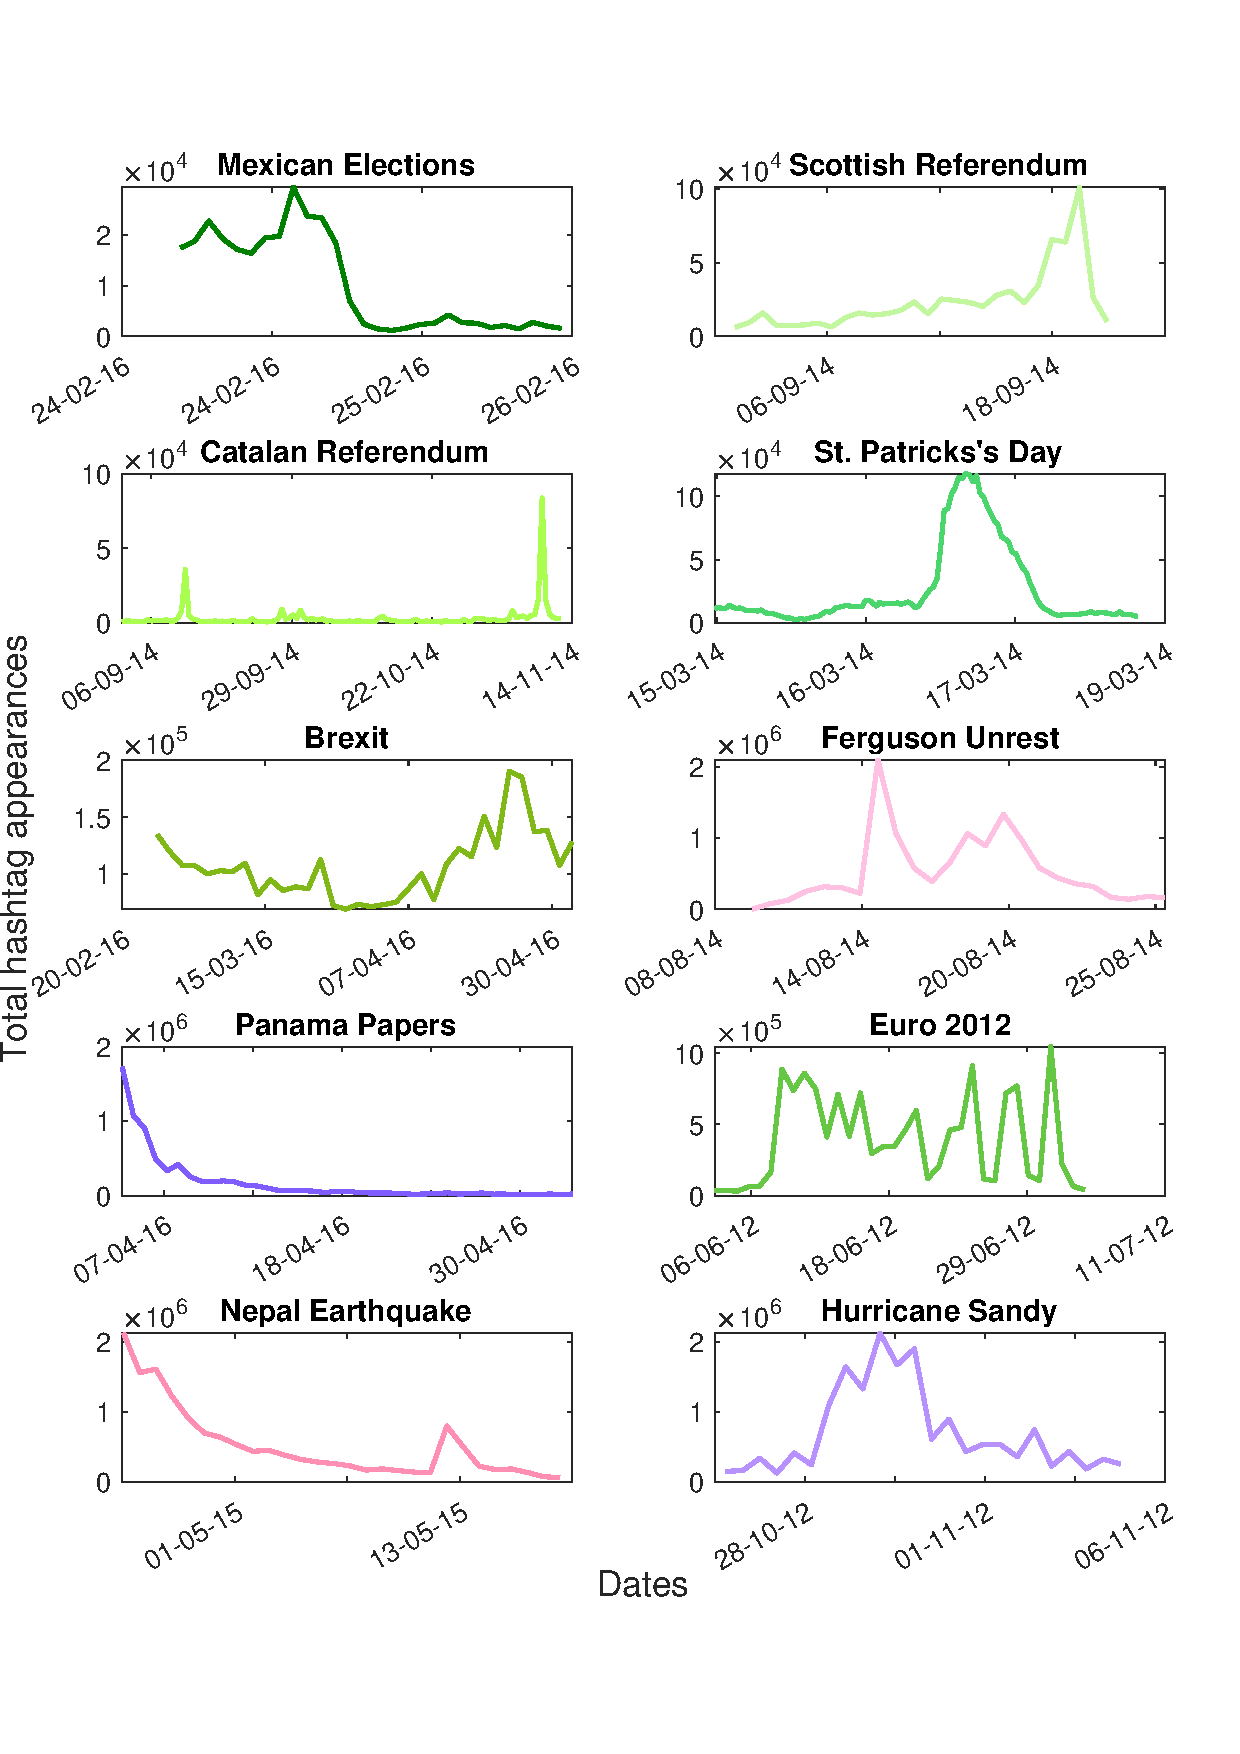
\includegraphics[width=\columnwidth]{figures/chp4/total_abuncances_vertical.pdf}
 \caption[Total hashtag abundances]{ Total hashtag appearances where the events of each dataset can be observed as peaks. }
\label{fig:4:totabun}
\end{figure}

Moreover, ecological patterns are usually defined within a community or are comparisons across communities.  These ecological communities are not straightforward to define, as dispersion and environmental factors can dilute their boundaries. Here, in order to represent communities, we have divided our datasets into a collection of posts referred to as bins. Our communities are then represented as different bins with constant sampling effort, that is, the number of posts where the hashtags can be found is fixed. Having a constant sampling effort prevents biases in the patterns. It is the equivalent of counting species in regular patches of land to characterize the community. The sampling effort, in our case, is represented as a certain number (or volume) of posts. A \textit{volume} bin consists of $V$ consecutive posts (Figure~\ref{fig:image}). We have selected a $V$ for each dataset according to its size and checked that our results remain almost unaffected by creating bins with different reasonable values of $V$. \\



%A bin is a population sample, i.e. a collection of posts that represent a community. \\

%Bins are generated in two ways depending on the nature of the patterns to detect.  If we are dealing with temporal patterns, we group the tweets according to their posting time (left-hand side of Figure~\ref{fig:image}). A bin then consists of the posts that have appeared during a fixed time interval of length $T$.  These time intervals are constant and consecutive, and each bin is thus refereed as a \textit{temporal} bin. Furthermore, we need a proxy when the patterns are not temporal but originally deal with abundances or species within a certain region or across different areas. For these patterns, space parallels with the sampling effort made to uncover the species. The sampling effort, in our case, is represented as a fixed number (or volume) of posts. A \textit{volume} bin consists of $V$ consecutive posts (right-hand side of Figure~\ref{fig:image}). 
%The bins are randomly sampled with replacement $B$ times, a technique known as bootstrapping. It is used to obtain better statistics of the dataset without assuming any underlying mechanism for the creation of the data. Bootstrapping is especially useful with small datasets, as a means to compensate for the distortions brought on by bursts of activity, which might not be entirely representative of the dataset. 
%Finally, we have checked that our results remain almost unaffected by creating abundance matrices with different reasonable values of $T$, and $V$.\\

Thus, a natural way to describe our datasets is employing a $H \times B$ abundance matrix,  where $H$ is the number of different hashtags in the dataset and $B$ is the total number of bins in which it has been divided. Each entry $n_{hb}$ represents the abundance, the number of posts of bin $b$ in which hashtag $h$ has appeared. Some key variables can be easily derived using the matrix representation. First, the total abundance of a bin $b$ is the column-sum $N_b = \sum_{h = 1}^H n_{hb}$. Notice that the number of hashtags in every volume bin is not constant. For each post, the number of hashtags may vary. The relative abundance of a hashtag is defined as  $x_{hb} = n_{hb}/N_b$, and it is normalized in such a way that $\sum_{h = 1}^H x_{hb} = 1$. Two other crucial observables are the mean relative abundance of a hashtag across all the bins $\bar{x}_h = \frac{1}{B} \sum_{b=1}^B x_{hb}$ and the total number of posts in the dataset $N = \sum_{b=1}^B N_{b} $.\\

To finish the data preparation, it is worth noticing a key difference between ecological and information ecosystems' data. Taking a simplified vision, in ecological experiments, there is usually not sufficient time, economic resources, and personnel to do a complete sampling. These problems usually result in subsampling and the impossibility to replicate experiments in different localities or habitats. For online social networks, the problem is on the other side of the spectrum. Data is abundant, albeit usually upon payment. We are said to be in the Big Data era for a reason. This means that even with pertinent data collection, we may end up with lots of spurious hashtags. For that reason, it is convenient to establish a method to discard those hashtags. As our datasets revolve around one or more events, and to reduce any noise that might have been caused by bots or misspelled hashtags, any hashtag that had been tweeted fewer than $75$ times was filtered out. We have verified that our results remain mostly unaltered when subjected to various filters.

%threshold for the number of bins in which a hashtag needs to appear to be considered in the analysis of patterns that are not sensitive to undersampling. When a hashtag appears at least in $50\%$ of the bins, we assume it is not spurious and has been involved in some discussion around the events. 

\begin{figure}[t]
     \centering
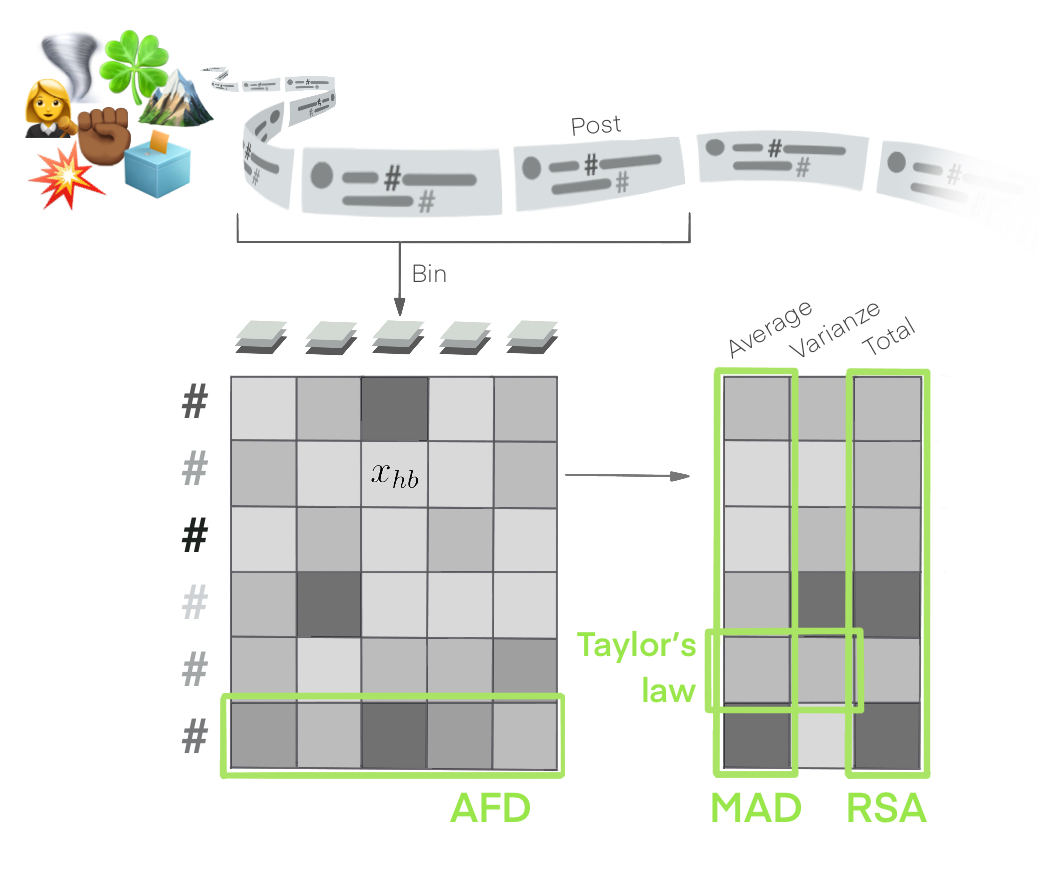
\includegraphics[width=\columnwidth]{figures/chp4/alagrilli.pdf}
 \caption[Data representation]{ The abundance matrix describes our datasets from the stream of posts of each event. After dividing the posts into bins, we aggregate the compositional data according to the pattern to uncover.}
\label{fig:image}
\end{figure}

%%%%%%%%%%%%%%%%%%%%%%%%%%%%%%%%%%%%%%%%%%%%%%%%%%%%%%%%%%%%%%%%%%%%%%%%%%%%%%%%%%%%%%%%%%%%%%%%%%%%%

\section{How: patterns for information ecosystems} %Define patterns, fitting, and particular data preparation methods if any
As we said, a large number of universal laws have been discovered in ecology. We have selected $6$ of them whose functional forms have been extensively discussed and have an ecological meaning that is transferable to information ecosystems, together with their applications in modeling and prediction. The patterns are the following: the abundance fluctuation distribution (AFD), Taylor's law, the mean abundance distribution (MAD), the relative species abundance distribution (RSA), the species-accumulation curve (SAC), and the short-term abundance change distribution (STAC). In the next paragraphs, the definition of these patterns is presented with a brief description of their importance. For a deeper review of the ecological implications of their forms, see Appendix~\ref{appen:patterns}.\\

%The regularities we have tested are defined for transversal data (see Figure~\ref{fig:image}), with the exception of the short-term abundance changes for longitudinal (temporal) data.

\paragraph{AFD:} The purpose of this pattern is to characterize the distribution of population abundance seen in different communities. To be more precise,  we refer to how the abundance levels of a single species change when it is measured in the different communities where it occurs. Ecologists have commonly  believed that population abundance is lognormally distributed \cite{May1975PatternsOS}, inspired by the fact that population growth is a multiplicative (rather than additive) process \cite{marquet2005scaling}. Moreover, a gamma distribution has also been postulated to describe the AFD and has obtained superior fits in some cases \cite{halley2002lognormality,grilli2020macroecological}. In the latter case, the probability species $h$ has a relative abundance $x$ in a bin is:
\begin{equation}
    \rho_h (x) = \frac{1}{\Gamma(\beta_h)} \left( \frac{\beta_h}{\overline{x}_h} \right)^{\beta_h}    \overline{x}^{\beta_h -1} \textrm{exp} \left( -\beta_h \frac{x}{\overline{x}_h} \right),
\end{equation}
where $\overline{x}_h$ is the mean (relative) abundance of species $h$, the parameter $\beta_h$ is its squared inverse coefficient of variation,  $\beta_h = (\overline{x}_h / \sigma_h)^2 $, and $\Gamma(\beta_h)$ is the gamma function.\\


\begin{comment}
Method:  
1) Choose the most abundant hashtag that is present in all bins 
	1.1) we just show one hashtag, and it is not the sampler (comprobar todo esto)
2)  Fit the relative abundance to gamma and lognormal (MLE maximum likelihood estimates). Why also checking lognormal? The gamma distribution is proposed, it is not derived.
3) Plot theoretical curve: Goodness of fit: chi2
4)  Log and Rescale the x-axis
\end{comment}


\paragraph{Taylor's law:} 
Empirical studies and models have observed that the variance in population abundance across communities $\sigma_h^2$ for many species follows a power law relationship with the mean population abundance $\overline{x}_h$ \cite{taylor1961aggregation,grilli2020macroecological}:
\begin{equation}
    \sigma_h^2 \sim \overline{x}_h^{\alpha}.
\end{equation}
The exponent $\alpha$ is fractional and lies between $1$ and $2$, with many species close to the extremes \cite{anderson1982variability}. It is of particular interest when the variance scales quadratically with the mean, which happens in microbial communities \cite{grilli2020macroecological}. This convergence of the exponent to $2$ can be an indicator of  stochasticity, or a consequence of non-trivial dynamics, such as spatial heterogeneity \cite{keeling2000simple}.


\paragraph{MAD:}  Apart from the scaling of the mean abundances, we have also looked at the mean distribution of all the hashtags in a dataset. The mean abundance distribution (MAD) is proposed to be lognormally distributed \cite{grilli2020macroecological}. If a hashtag is chosen at random, the probability of having a mean abundance $\overline{x}$ is:
\begin{equation}
    p(\overline{x}) = \frac{1}{\sqrt{2 \pi \sigma^2} \overline{x}}
    \textrm{exp} \left( -\frac{(\textrm{log}\overline{x} - \mu)^2}{2\sigma^2} \right),
\end{equation}
where $\mu$ and $\sigma$ are the parameters of the lognormal distribution, which are unique for each dataset. The mean relative abundance values are obtained in the same way as for Taylor's law. 

\paragraph{SAC:} The species-accumulation curve links the number of different species $s$ with the size of the population in which they are found. This pattern fundamentally represents how the number of observed species scales with sampling effort. %Since for us, hashtags play the role of species, then the number of different posts containing a certain hashtag represents its population size. 
We can redefine the SAC for information ecosystems as a pattern that relates the number of distinct hashtags with the total number of posts in which they are looked at, i.e. the scale ($N$). 

In ecology, depending on the spatial scales, the SAC shows different behaviors: linear for local and large areas, and a power-law relationship ($s \sim A^z$) for intermediate scales \cite{azaele2016neutral}. A precise form can be proposed if we assume that the sampling of the hashtags is governed by a gamma-distributed AFD \cite{grilli2020macroecological}. In that case, the empirical expected mean value is 
\begin{equation}
    \langle s(N) \rangle =
    s_{tot} \left( 1 - \int d\eta \frac{\textrm{exp}\frac{-(\eta-\mu)^2}{2\sigma^2}}{\sqrt{2\pi \sigma^2}} 
    \left(\frac{\beta}{\beta + e^{\eta}N}\right)^{\beta} 
    \right). \label{eq:SAC}
\end{equation}
This functional form can be applied if we assume that the previous patterns hold. Specifically, the values of $\mu$ and $\sigma$ represent the parameters estimated from the lognormal distribution of the MAD, while $\beta = \frac{1}{H}\sum{\beta_h}$ is the mean of the beta parameter of the AFD gamma distribution of each hashtag.
%To compare the empirical scaling with the preceding expression, we have used parameters of other patterns, effectively binding them. The values of $\mu$ and $\sigma$ obtained from the lognormal MAD, and $\beta = \frac{1}{H}\sum{\beta_h}$ is the mean gamma AFD's parameter over all hashtags. 
 
\paragraph{RSA:} Within most natural communities, only a few species constitute the majority of the individuals found there and lots of species are in small numbers. That is, there are numerous rare species and only a few abundant species, making the relative species abundance distribution (RSA) highly skewed \cite{preston1948commonness,brown1995macroecology}. The RSA patterns have been well described with negative binomial or lognormal distributions, which are grounded in the theoretical framework of the neutral theory of ecology \cite{hubbell2001unified,volkov2007patterns}. Note that the RSA is looking at the whole community, classifying species according to their abundance. Contrarily, the AFD is another pattern that involves distributions of abundance, but in that case, the focus is on how the abundance of one single species varies across regions.

\paragraph{STAC:} Finally, the short-term abundance change is defined as the logarithm of the ratio of species abundances in consecutive temporal measures:
\begin{equation}
    \lambda_{hb} = \textrm{log} \left( \frac{x_{h b+1}}{x_{hb}} \right),
\end{equation}
where the relative abundance of the next time frame is denoted as $x_{hb+1}$ for convenience. The probability of a certain change averaged over all successive measurements and aggregating species  follows the Laplace distribution: 
\begin{equation}
    p(\lambda) = \frac{1}{2\gamma} \textrm{exp} \left( \frac{- |\lambda - u|}{\gamma} \right),
\end{equation}
where $u$ is the mean and $\gamma > 0$ is the scale parameter of the distribution. This pattern is well spread, being found in ecological communities \cite{marquet2005scaling}, bacterial population dynamics \cite{ji2020macroecological}, and even companies and universities \cite{stanley1996scaling,plerou1999similarities}.

Unlike the other patterns discussed, the STAC is a temporal pattern because studies abundance changes through time. In a microbial sample, for instance, the fluctuations in abundance are measured at fixed time intervals through the experiments \cite{ji2020macroecological}. Our datasets have a temporal component too since posts are created at a certain moment. Fortunately, we have access to that information and can use it to create a bin that suits better to this pattern. Here we group the tweets in an alternative binning according to their posting time. A bin consists now of the posts that have appeared during a fixed time interval of length $T$.  We then compare the fluctuations in abundance between consecutive bins. \\ 
%- What do we do when a bin has zero abundance? We  take into account the species, but do not calculate $mu_k(t) and mu_k(t-1)$

The parameters of all the patterns have been obtained using  maximum likelihood estimation. We have also tested whether our empirical patterns align with the theoretically proposed functional forms. The results of the statistical tests can be found in Appendix~\ref{appen:patterns}.
%%%%%%%%%%%%%%%%%%%%%%%%%%%%%%%%%%%%%%%%%%%%%%%%%%%%%%%%%%%%%%%%%%%%%%%%%%%%%%%%%%%%%%%%%%%%%%

\section{Patterns uncovered}

After presenting the patterns, we proceed to search for them in our datasets. We find that our empirical data is compatible with the ecological functional forms of the patterns, regardless of the type of discussion, since the expected shapes of all patterns are identified across every dataset. In addition, there are no significant deviations among the datasets despite their variations in size and nature. For example, one could have found no connection between mean abundance and variance, or a non-polynomial relation contrary to Taylor's law. Instead, we find the same laws found in natural ecosystems. This indicates that the patterns are consistent for information ecosystems too, and can capture the common rules of the multiple datasets. The next Subsections show every pattern and discuss this striking resemblance.\\

To start with, the AFD has a common shape across all datasets. In Figure~\ref{fig:4:AFD}, the cumulative probability for the most abundant hashtag is plotted with the predicted gamma and lognormal distributions' fits, showing that the empirical data is compatible with both of them (the results of their statistical tests are in Appendix~\ref{appen:patterns:tests}).  Since the AFD follows a consistent pattern, when the abundance distribution of a particular hashtag is distorted, it could indicate that an external force is at play. By identifying deviations from this pattern, we may be able to uncover hashtags that are being boosted by unknown mechanisms.\\

\begin{figure}[h!]
    \centering
    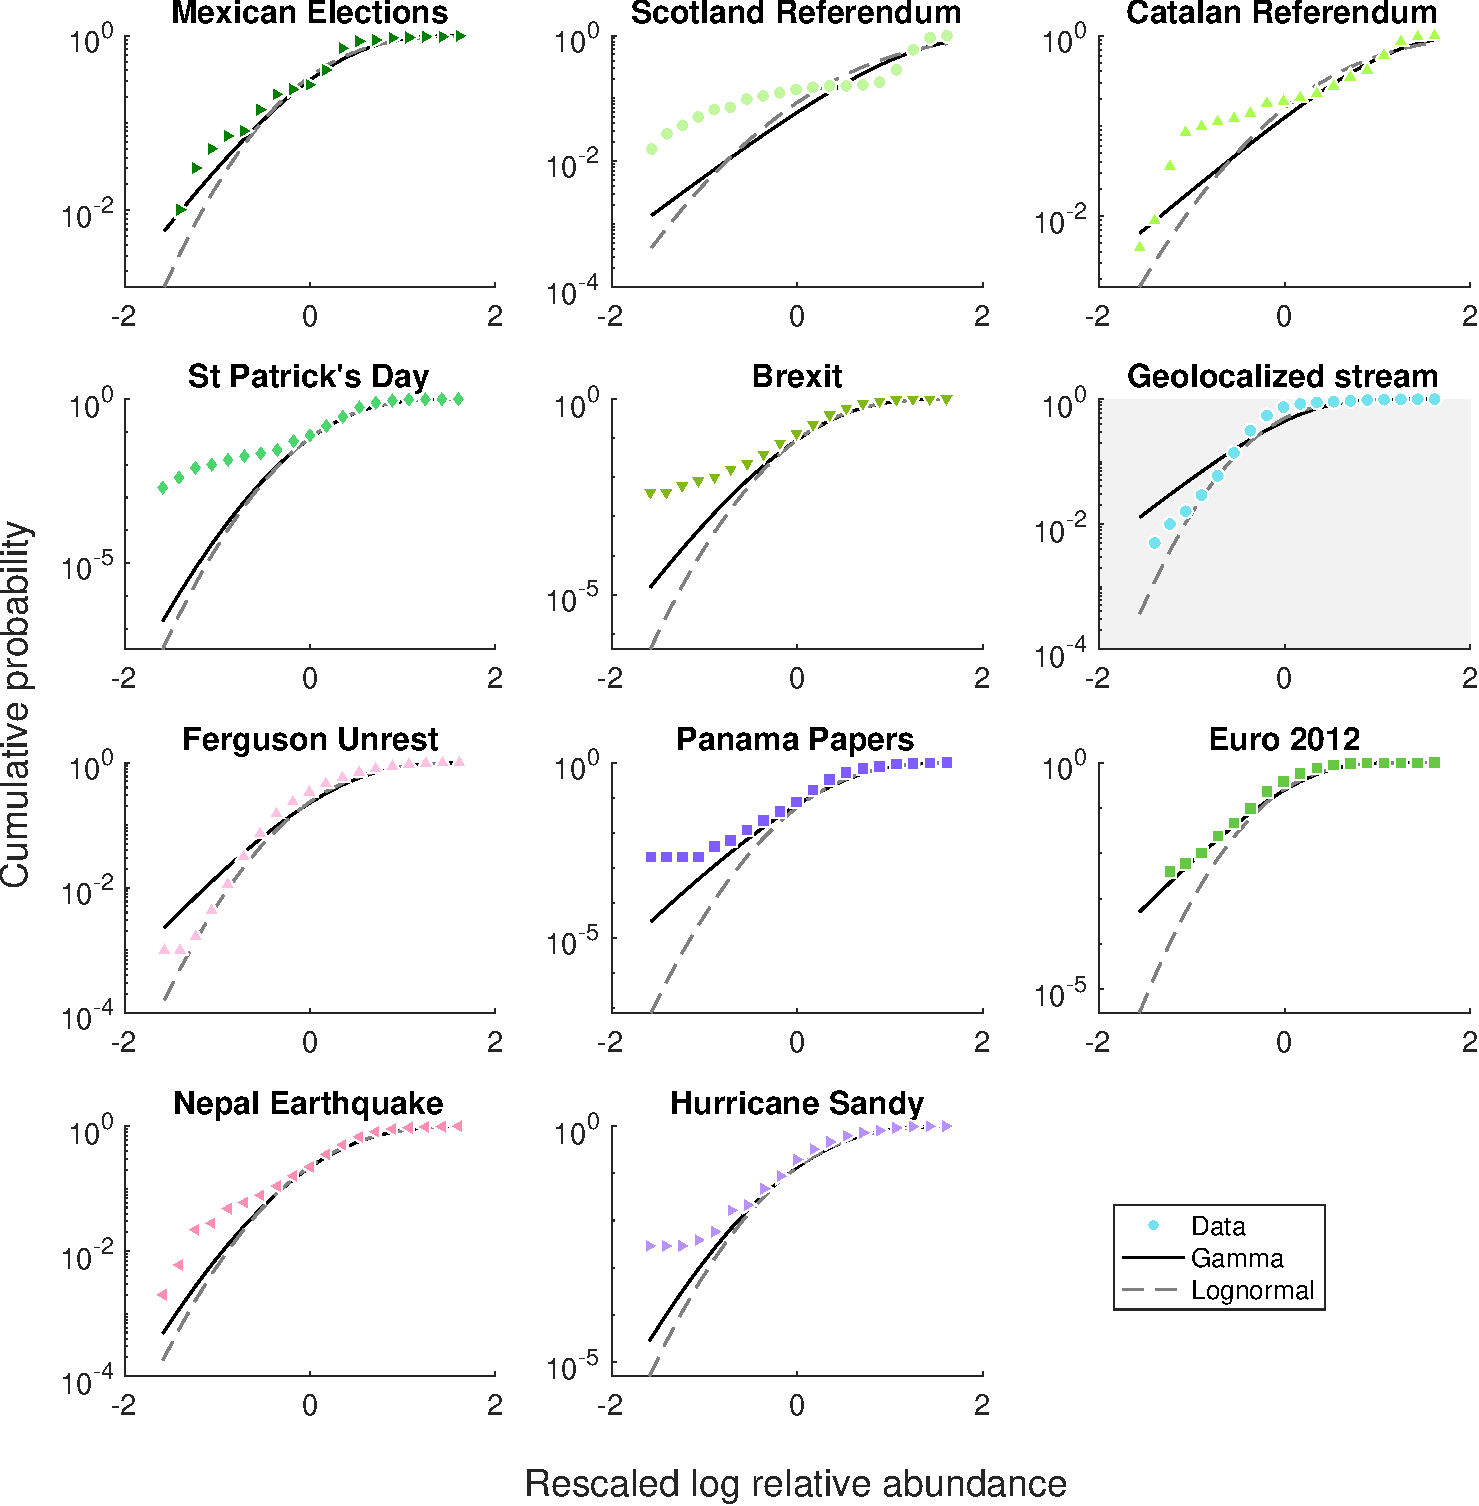
\includegraphics[width=\textwidth]{figures/chp4/AFD_tweet_RemSam.pdf}
    \caption[AFD]{AFD: Across each dataset, the distribution of abundances share a common shape. The datasets are sorted by the total number of different hashtags in ascending order. Greenish markers belong to expected events, pinkish to unexpected events. The sample which does not belong to any event (UK random) is in blue and hereinafter highlighted in gray for comparison. Relative abundances are rescaled to have zero mean and variance of one per bin.}
    \label{fig:4:AFD}
\end{figure}

Large abundances are particularly well described with these distributions. And among the parts that deviate from the distributions, the most usual feature is that small abundances are lower than expected. This indicates that hashtags have less extremely low abundances and could be a finite-size effect since the fluctuations in abundance are constrained by the finite amount of posts per bin. Interestingly, we find a complementary tendency in ecological data: the skewness is less than that expected, implying fewer extremely high values \cite{halley2002lognormality}. \\



%Among all the patterns, the AFD presents the highest variability, as some hashtags that are not the most abundant present other functional forms (see Figure X). The deviations may be a consequence of their hashtags frequencies, realization sizes, and of course, the existence of underlying generative processes.

Next, the mean relative abundance of hashtags across the bins in which datasets are divided scales with their variance following a power law (Figure~\ref{fig:4:TAY}): Taylor's law. An exponent close to $2$ arises consistently in all our datasets, suggesting that hashtags in online social networks follow a common dynamics that does not depend on either particular discussions or their size. The fit of Taylor's law exponents is shown in Table~\ref{tab:chp4:taylor}, where it can be observed that they are very similar. \\



\begin{table}[h] 
\caption{Estimated exponents across datasets for Taylor's law.}
\centering
\begin{tabular}{l c c c c } 
\hline 
Dataset &  $\alpha$ & $95\%$ CI & R \\ \hline \hline 
Mexican Elections & 1.895 & (1.857, 1.933) & 0.840 \\ \hline 
Scotland Referendum & 1.957 & (1.878, 2.036) & 0.610 \\ \hline 
Catalan Referendum & 1.874 & (1.816, 1.932) & 0.817 \\ \hline 
St Patrick's Day & 1.906 & (1.869, 1.943) & 0.689 \\ \hline 
Brexit & 1.858 & (1.826, 1.890) & 0.751 \\ \hline 
Geolocalized stream & 1.942 & (1.880, 2.004) & 0.718 \\ \hline 
Ferguson Unrest & 1.818 & (1.779, 1.856) & 0.804 \\ \hline 
Panama Papers & 1.812 & (1.686, 1.938) & 0.865 \\ \hline 
Euro 2012 & 1.933 & (1.823, 2.043) & 0.879 \\ \hline 
Nepal Earthquake & 1.865 & (1.848, 1.882) & 0.841 \\ \hline 
Hurricane Sandy & 1.882 & (1.864, 1.900) & 0.835 \\ \hline 
\end{tabular} \label{tab:chp4:taylor}
\end{table} 


%\begin{figure}[t]
 %   \centering
  %  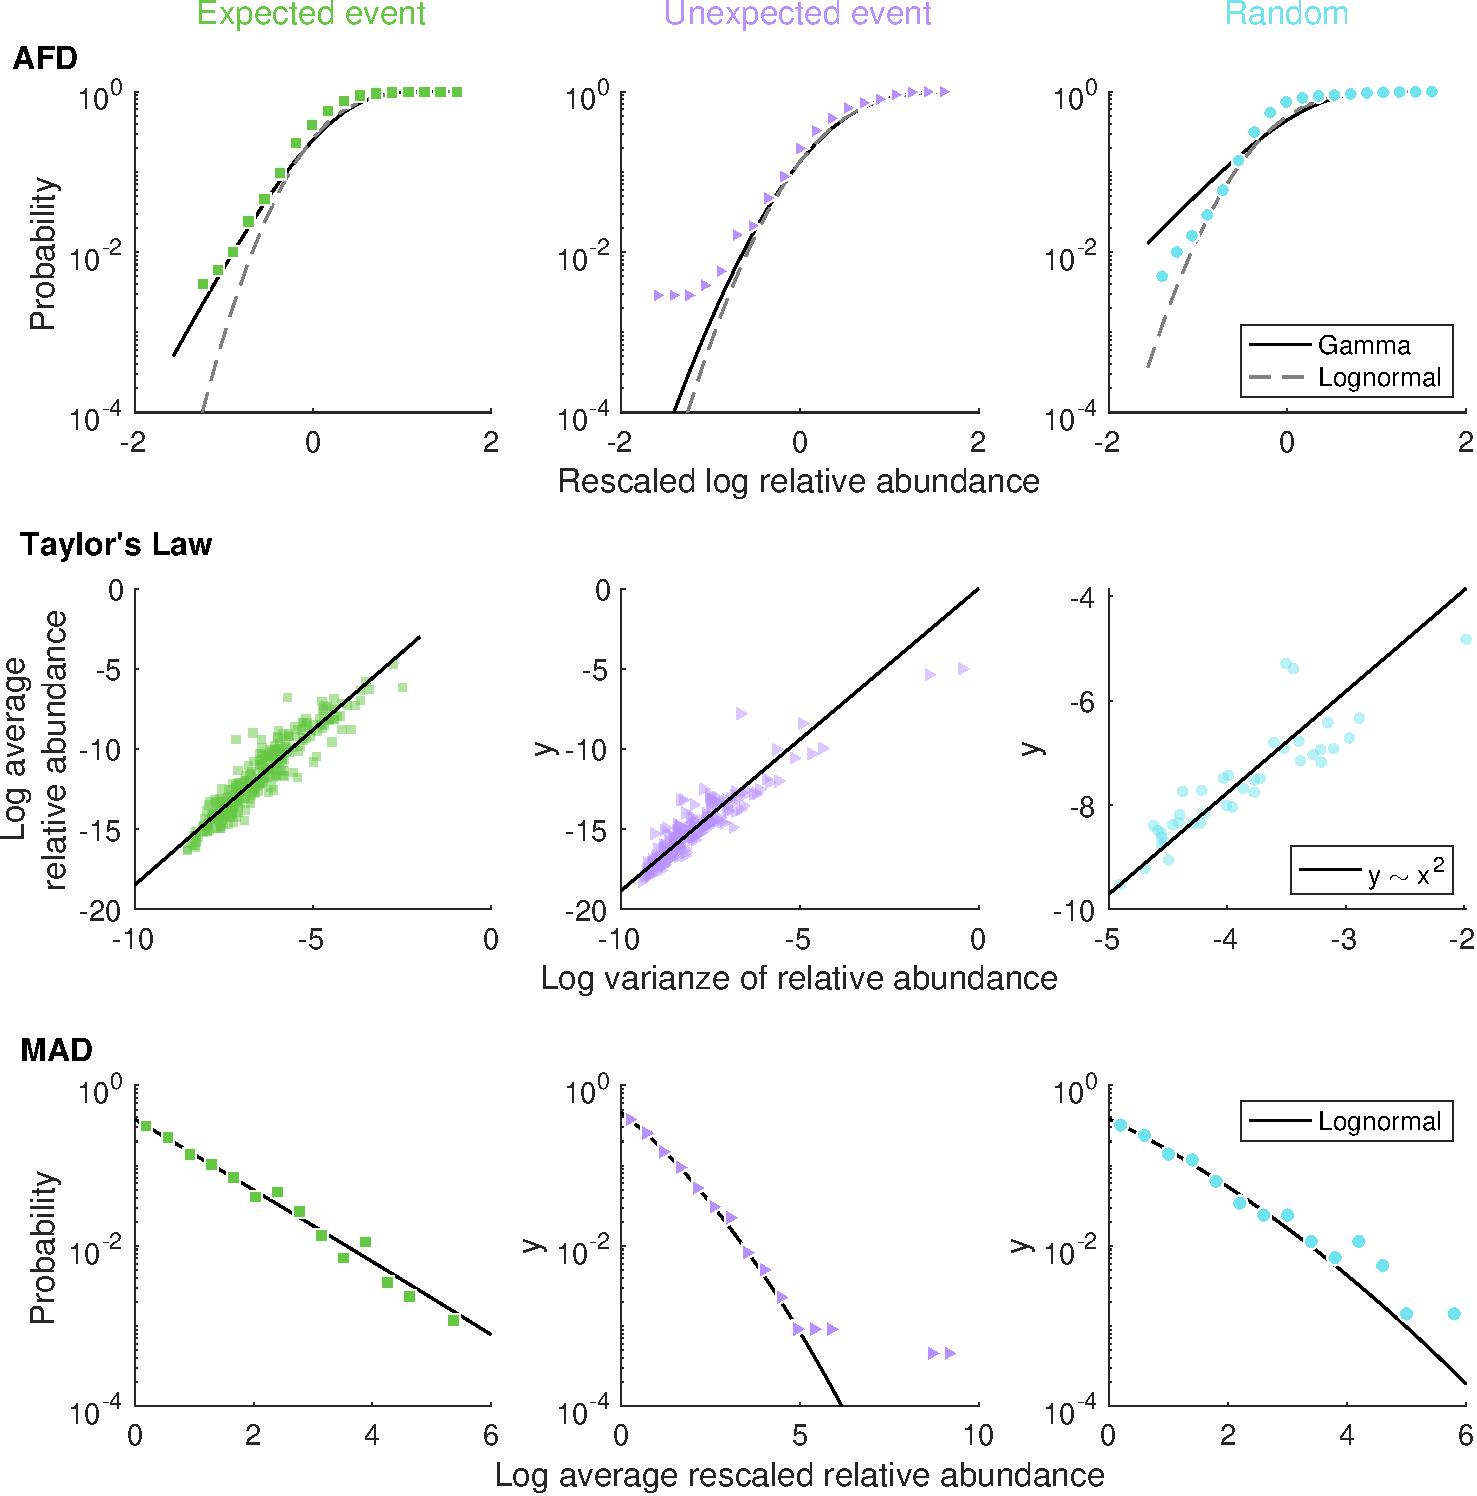
\includegraphics[width=\textwidth]{figures/chp4/Figure_Patterns1.pdf}
   % \caption[AFD, Taylor's law and MAD]{Caption}
    %\label{fig:AFD_TAY_MAD}
%\end{figure}

\begin{figure}[h!]
    \centering
    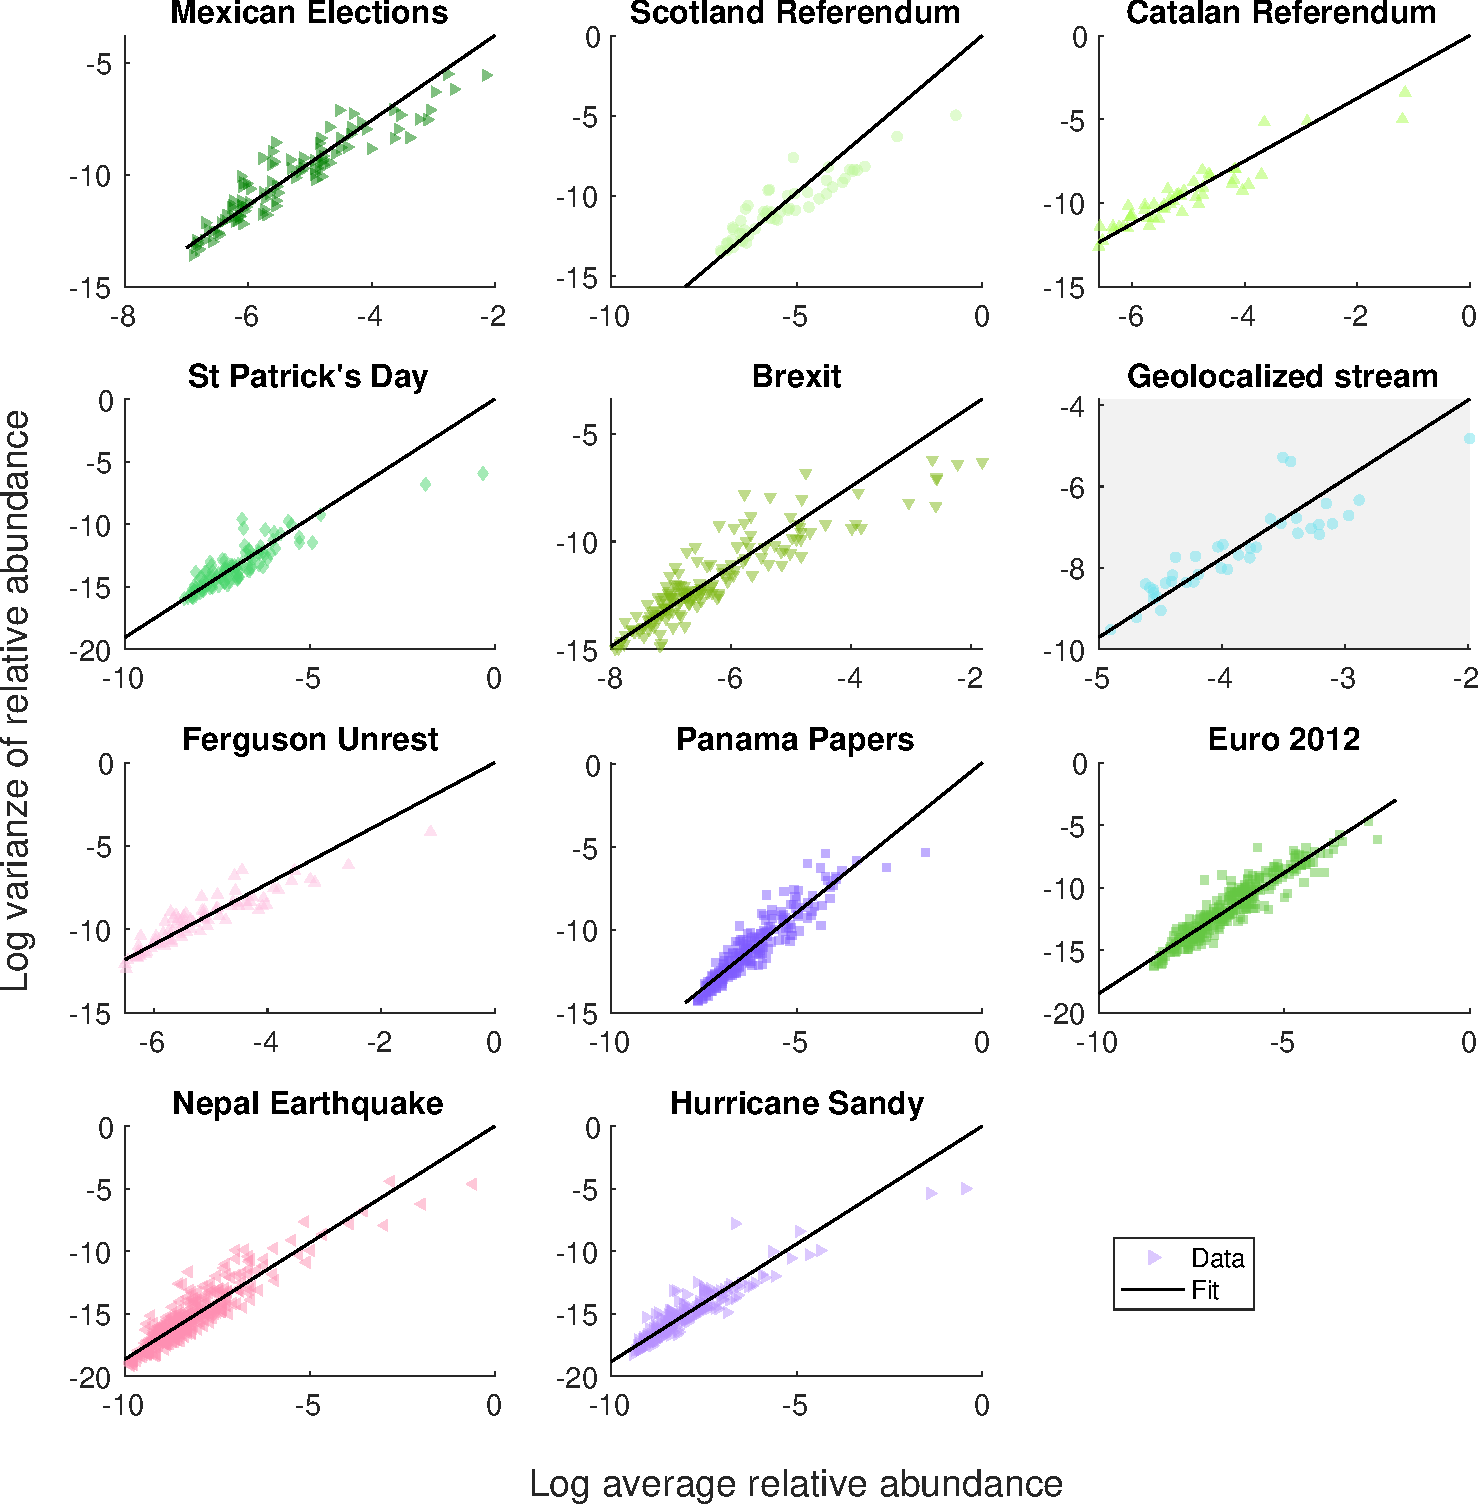
\includegraphics[width=\textwidth]{figures/chp4/TAYLOR_tweet_RemSam.pdf}
    \caption[Taylor's law]{Taylor's law: The variance of the abundance of hashtags over bins increases with the mean relative abundance as a power law of the from $\sigma_h^2 \sim \overline{x}_h^{\alpha}$. This relationship is consistent among all datasets with similar exponents. In the Panels, each point represents a hashtag. }
    \label{fig:4:TAY}
\end{figure}

Moving to the next pattern, when we plot the distribution of mean relative abundances (MAD), we observe that a lognormal distribution is compatible with them in all datasets (Figure~\ref{fig:4:MAD}). The shapes of the distributions vary from dataset to dataset, but a lognormal form is the best fit for all the datasets although with different values of $\mu$ (Table~\ref{tab:MAD}), like in ecological and microbial communities. General distributions in patterns like MAD and AFD, which remain consistent despite differences in details, can be applied in models to incorporate variability in their parameters. For example, the carrying capacity \cite{grilli2020macroecological} or food-webs interactions \cite{anderson1982variability} would not be constant, but random variables drawn from the corresponding distributions. Even though this approach would not capture all the variability of these parameters, it would still be more realistic than completely ignoring it. \\

 \begin{figure}[ht!]
    \centering
    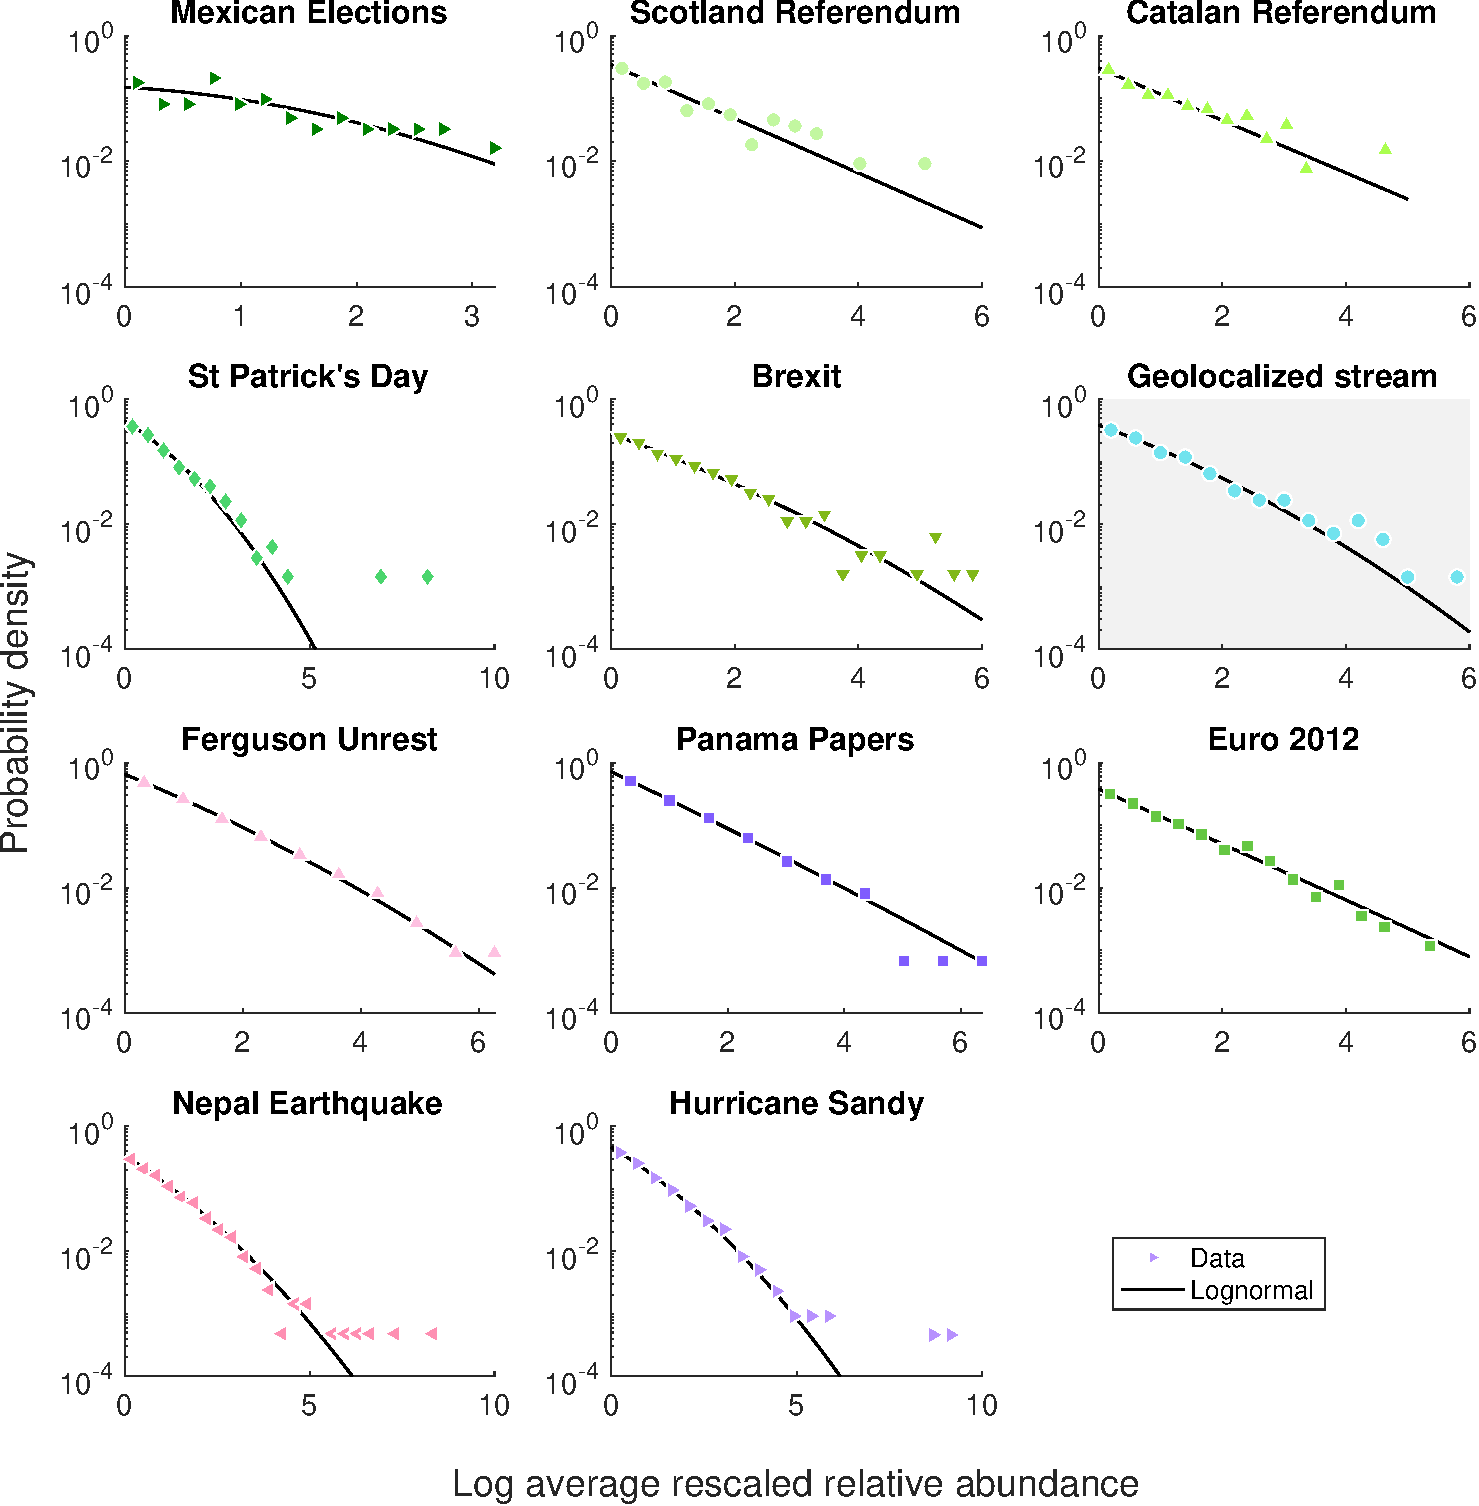
\includegraphics[width=\textwidth]{figures/chp4/MAD_tweet_RemSam.pdf}
   \caption[MAD]{MAD: The fit of the mean abundances closely follows a lognormal distribution. It is only performed over the positive values of their logarithm because the empirical MAD shows a lower cutoff established by sampling. The cutoff is based on the possibility that rare hashtags will never be found in a finite number of samples \cite{grilli2020macroecological}.}
    \label{fig:4:MAD}
\end{figure}

Moreover, a feature that we only see in some datasets related to events is that the most abundant hashtags have a mean relative abundance higher than dictated by lognormality.  Interestingly, the random-sampling dataset does not have this fat tail, indicating that it may be a sign of other processes going on in the former datasets that inflates certain hashtags.\\
%There is also a remarkable resemblance between these distributions and the frequency distribution of hashtags over the whole system, which means that the process generator of the abundances does not dilute the information about the recurrence of hashtags. Then, in a dataset with a high number of uncommon hashtags, we expect to find a high number of low-abundance hashtags.

For the species-accumulation curve (SAC), all the datasets present some part of the power-law relationship characteristic for intermediate scales (Figure~\ref{fig:4:SAC}). Some of them also start to saturate, meaning that we have sampled a considerable part of the discussion in those cases. The theoretical prediction for this pattern (Eq.~\ref{eq:SAC}) overall matches the empirical trends.\\


 %Within most natural communities, only a few species constitute the majority of the individuals and lots of species are in small numbers. That is, there are numerous rare species and only a few abundant species, making the relative species abundance distribution (RSA) highly skewed \cite{preston1948commonness,brown1995macroecology}. The RSA patterns have been well described with binomial or lognormal distributions, which are grounded in the theoretical framework of the neutral theory of ecology \cite{hubbell2001unified,volkov2007patterns}. These functional shapes depend on the type of scale considered, intrinsically connecting the RSA with the SAC \cite{azaele2016statistical}.
 In turn, the distribution of the abundance of hashtags (RSA) is consistent across all datasets and resembles the two proposed ecological distributions. There are few common hashtags with high abundance, but lots of hashtags are very uncommon. The same sweked RSA has also been found in some human communication systems such as emails, texts, and Twitter conversations \cite{tovo2021upscaling}. \\
 
 Remarkably, the UK random dataset, where there is not any main discussion to which those abundant hashtags can belong,  follows the same pattern as event-related datasets. Being that robust, a deviation from this trend could help in providing an estimate of the number of hashtags, and hence discussions, that a social network could host. \\


\begin{figure}[h!]
    \centering
    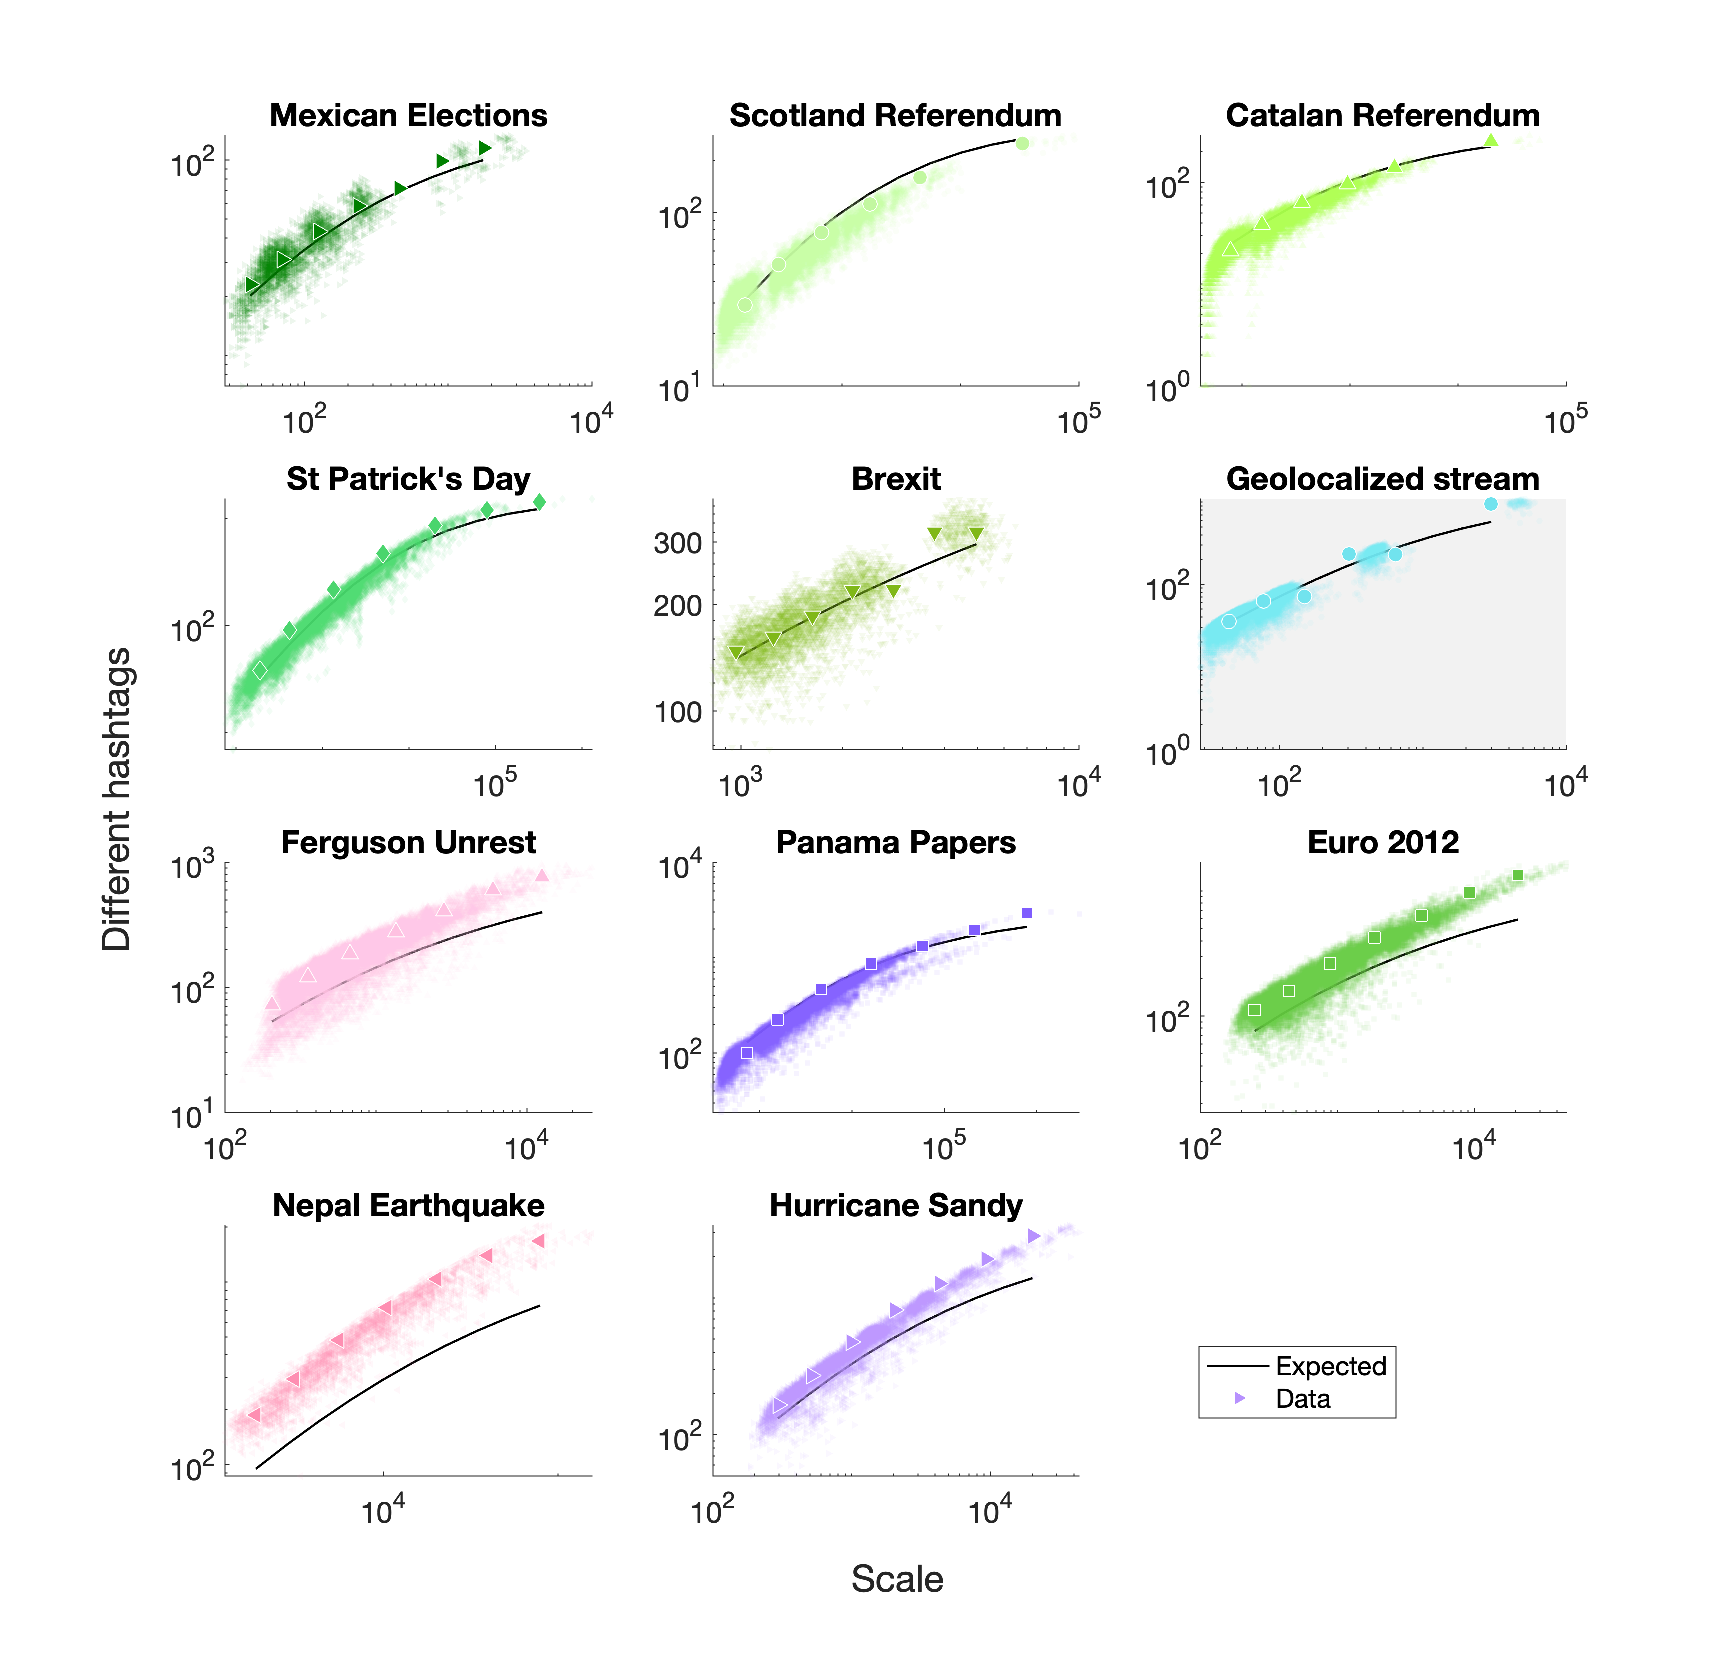
\includegraphics[width=1.1\textwidth]{figures/chp4/SAC_tweet_RemSam.pdf}
    \caption[SAC]{SAC: The species-accumulation curve for all datasets has a similar growth. Small points are bins, each of which with a different number of tweets (a proxy of scale). Larger points are averages over }
    \label{fig:4:SAC}
\end{figure}


\begin{figure}[h!]
    \centering
    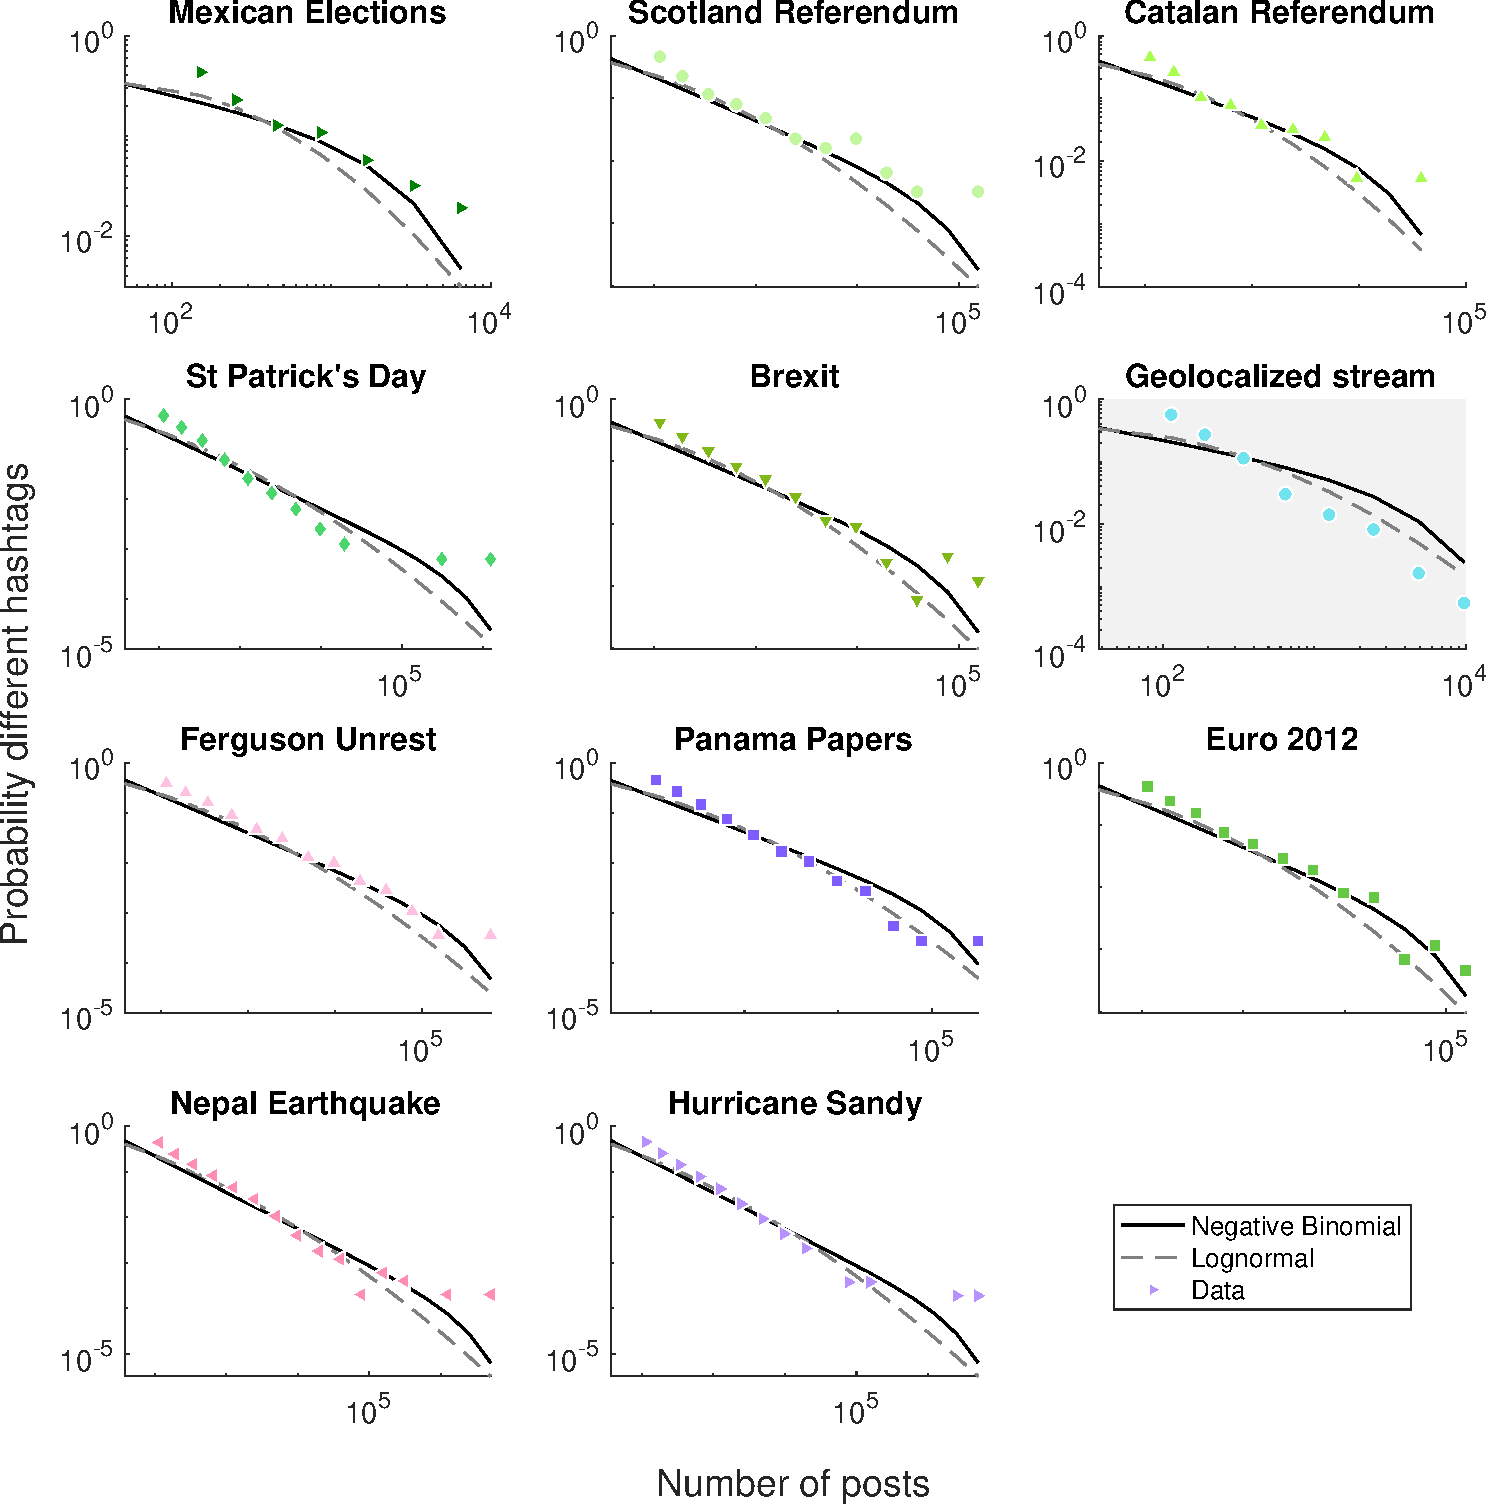
\includegraphics[width=\textwidth]{figures/chp4/RSA_tweet_RemSam.pdf}
    \caption[RSA]{RSA: The probability of hashtags having a certain abundance follows a consistent form across all the datasets. It is plotted on a logarithmic scale, where each interval is twice the preceding one, following the classic work of \cite{preston1948commonness}. }
    \label{fig:4:RSA}
\end{figure}

For the STAC all the datasets reproduce a Laplace distribution (Figure~\ref{fig:4:STAC}). The abundance changes in our datasets share two common characteristics with the STAC of ecological communities: they are remarkably symmetrical and their mean $u$ tends to zero (Table~\ref{tab:STAC}). Thus, exactly as many hashtags are decreasing their abundance as they are increasing over the  recorded period. Such a pattern is compatible with a symmetric and zero-sum game as a generative mechanism for the data. Specifically, this zero-sum game is related to species competing for a finite set of resources \cite{marquet2005scaling,ji2020macroecological}. Moreover, it has been proven that the dynamics going on is compatible with a zero-sum game where the resource the different actors are competing for is the finite attention of the users \cite{gleeson2014competition,plata2021neutral,palazzi2021ecological,calleja2021quantifying}, so this pattern reaffirms with our current understanding of human behavior in online social networks.\\

Finally, it is worth mentioning another connection between the distribution of temporal changes in ecological and human systems. If the population mean abundance (MAD) follows a lognormal distribution, the STAC is theoretically expected to be Gaussian distributed. Even though the MAD of these systems is compatible with a normal distribution, a Laplace distribution for the STAC has been found not only in nature but also in artificial scenarios such as human institutions, from the growth rates of companies to countries’ gross national
product \cite{marquet2005scaling}. This ubiquitous presence suggests the existence of universal principles governing the growth dynamics of complex adaptive systems that are engaged in acquiring, transforming, and storing information, materials, or energy. \\


\begin{figure}[t]
    \centering
    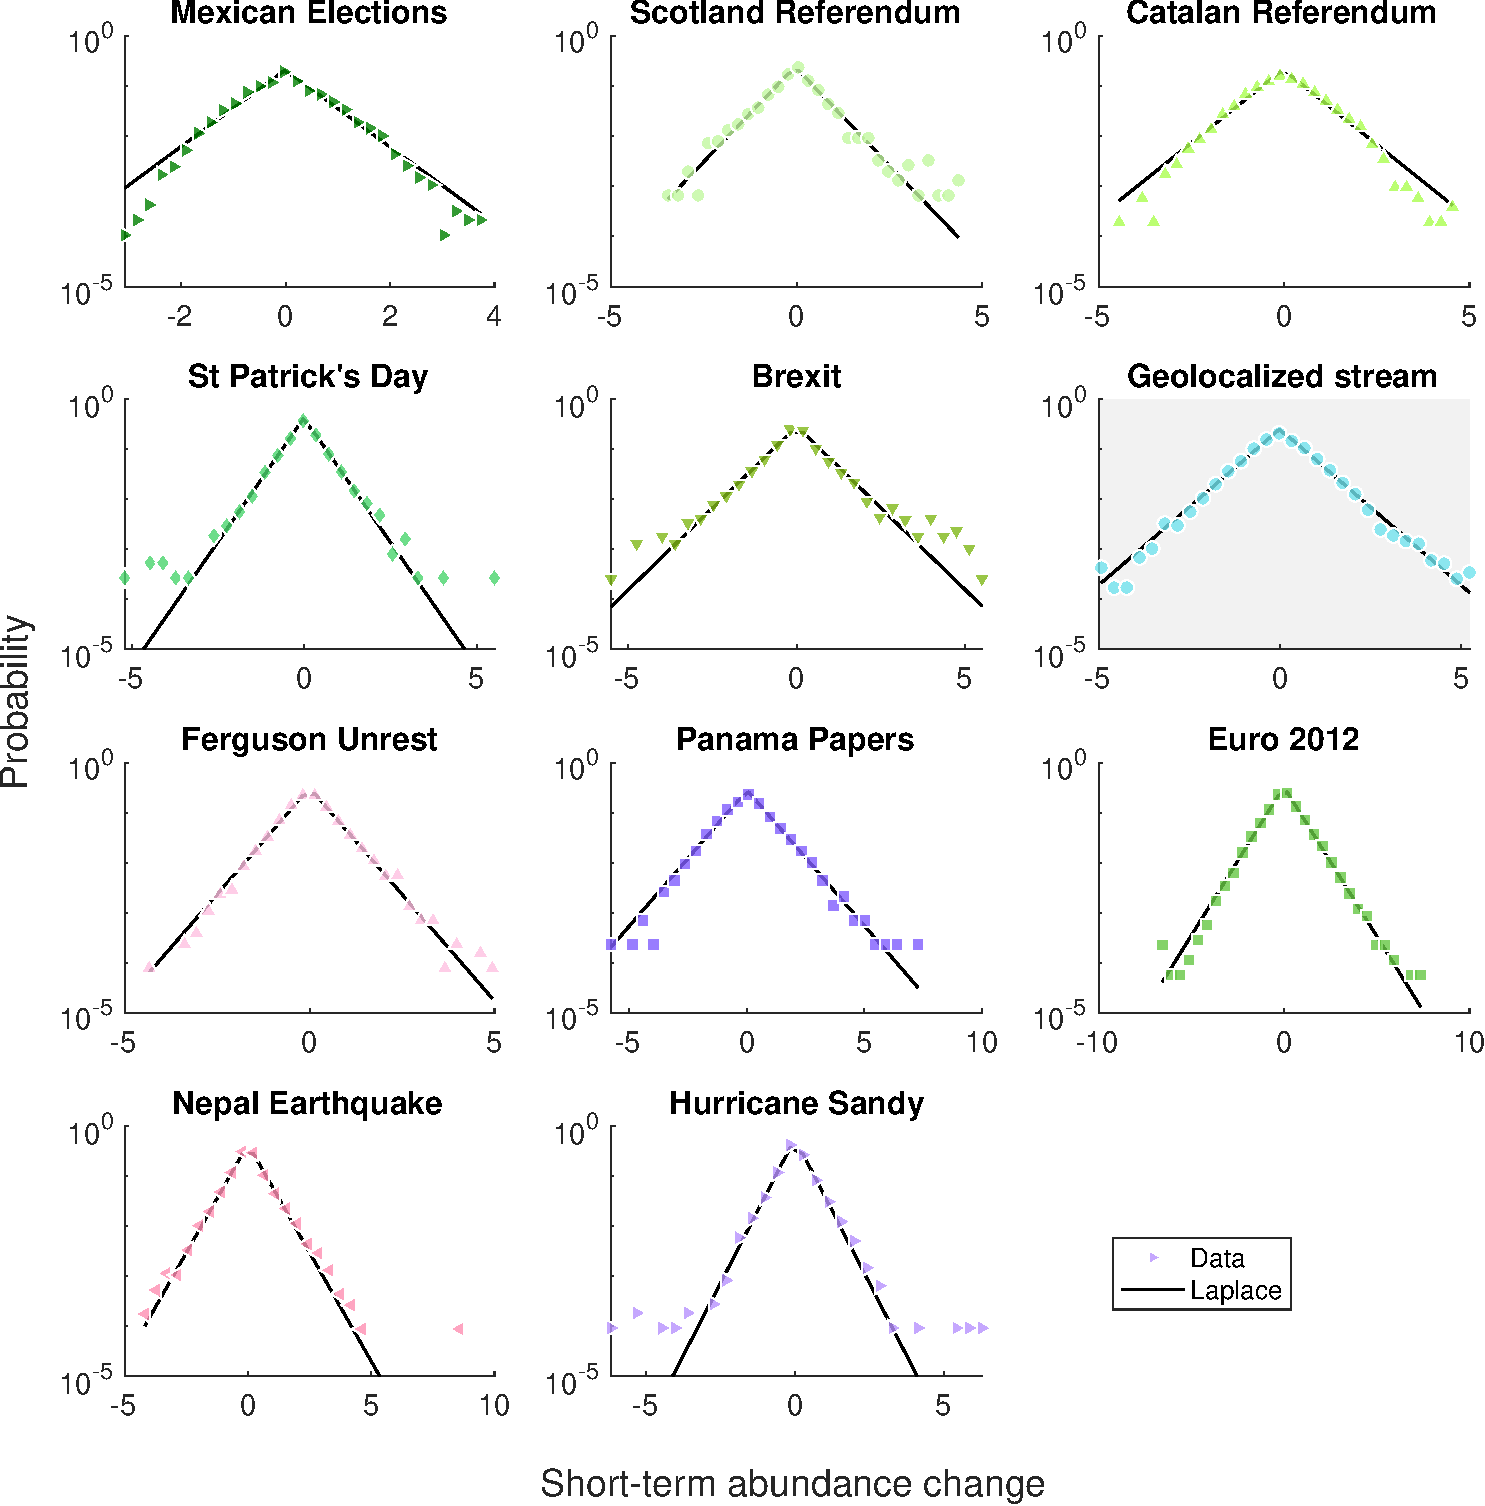
\includegraphics[width=\textwidth]{figures/chp4/STAC_tweet_RemSam.pdf}
    \caption[STAC]{STAC: The distribution of temporal fluctuations fits with the Laplace distribution also found in ecological and social settings.}
    \label{fig:4:STAC}
\end{figure}


\section{Multinomial random sampling}
Once we have demonstrated that information ecosystems present the same universal laws observed in natural ecosystems, we go one step further in trying to understand their origin. In particular, there are two key ingredients to explain the emergence of patterns. One of them is discovering how the frequencies of each hashtag are generated. Why do we have a few very abundant hashtags and lots of rare hashtags? The second ingredient is determining how users choose what hashtags to post. We focus only on this latter aspect and generate synthetic communities with the same features as the observed ones but based on a null model. Specifically, we employ multinomial sampling. Starting from the hashtags' frequency distribution this method \cite{lego} generates random bins. We then calculate the same patterns from these resampled random bins and compare their characteristics with the original patterns (Figure~\ref{fig:4:randomSampling}).
%This method generates new bins by only assuming that hashtags appear randomly according to a fixed frequency. 
Besides, the model is neutral, which implies that all hashtags are equal in the eyes of the user.\\

Regarding how the model is implemented, we can replicate an empirical bin $b$ creating a random sample (with replacement) of size $N_b$, in which the probability that a set of hashtag abundances $ \{n_{h}\}$ occurs is given by:
\begin{equation}
    P(n_1, ... , n_H, N_b, f_1, ... , f_H) = \frac{N_b!}{\prod n_h!} \prod f_h^{n_h}
    \label{eq:multinomial}
\end{equation}
 where the frequency of a hashtag in the whole dataset is $f_h = \frac{1}{N} \sum_{b=1}^B n_{hb}$, and hence the probability of a new hashtag extraction is proportional to its global abundance $\sum_{b = 1}^B n_{hb}$. By doing this resampling for every bin of a dataset, we obtain a new random abundance matrix with the same size of the original one.

\begin{figure}[t]
    \centering
    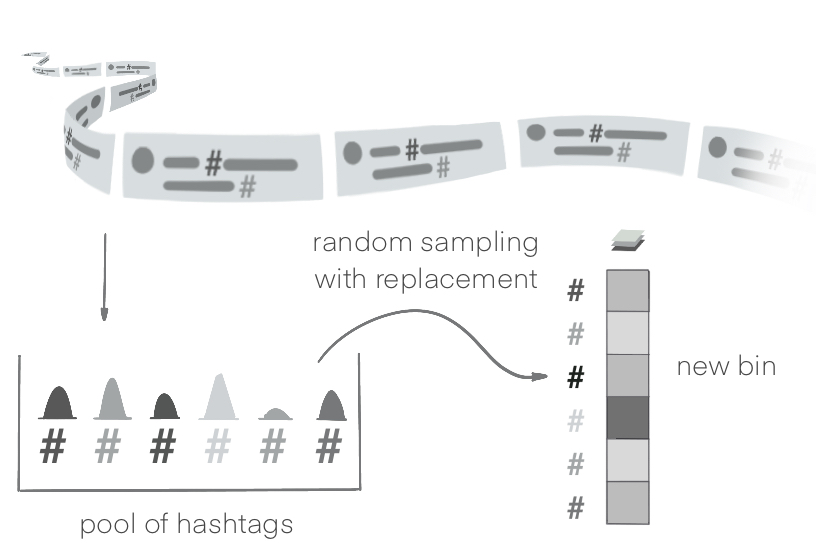
\includegraphics[width=0.8\textwidth]{figures/chp4/randomSampling.pdf}
    \caption[Multinomial random sampling of posts]{Resample procedure: for every empirical dataset, we have calculated the hashtag frequencies and used them to resample each bin conserving the total number of hashtags found originally there.}
    \label{fig:4:randomSampling}
\end{figure}

\subsection{Confronting patterns}
By comparing the empirical patterns to the prediction generated by the multinomial random sampling, we can determine whether other factors besides hashtag frequency are driving the hashtag sampling. To do so, we have created $20$ resampled abundances matrices from our largest dataset and plotted their distributions together with the empirical ones in Figure~\ref{chp:4:fig:Lego}.\\

The analytical predictions based on Eq.~\ref{eq:multinomial} for some patterns (in Appendix~\ref{appen:patterns:eqs}) already tell us that an exponent one in Taylor's law is expected, which is precisely what we found with resampled data. Regarding the MAD, the multinomial data perfectly matches the frequency distribution (Figure~\ref{fig:appen:LegoAux}), which in turn remains close to the empirical distribution of mean abundances. Since the empirical MAD also reproduced the frequency distribution up to some extent, it is not a relevant pattern to distinguish deviations related to other processes and constraints in the datasets. This same reasoning can be applied to the RSA and SAC. The patterns that deal with distributions of fluctuations --AFD and STAC-- are expected to be more sensitive to external factors. In fact, for the AFD, the resampled distributions in Figure~\ref{chp:4:fig:Lego} present in general a higher probability of fluctuations. For the STAC, on the other hand, the short-term fluctuations are smaller than the empirical counterpart. Besides, in resampled bins, the dispersion of Taylor's law and SAC is reduced. However, this is not something remarkable since the random sampling has no exogenous noise. \\

Regarding the theoretical fits, some  patterns of the resampled bins have the same  peculiarities as the empirical patterns for online social networks: the AFD is fatter than the theoretical functional forms for small abundances --see Figures~\ref{fig:4:AFD} and~\ref{fig:appen:LegoAux}-- and both RSA present heavy tails --see Figures~\ref{fig:4:RSA} and~\ref{fig:appen:LegoAux}. \\

 %Multinomial AFD. The new bins are created with a different number of instances, accordingly to the bin from which we have taken the hashtags' frequencies, so a Binomial fit is not expected.

\begin{figure}[t]
    \centering
    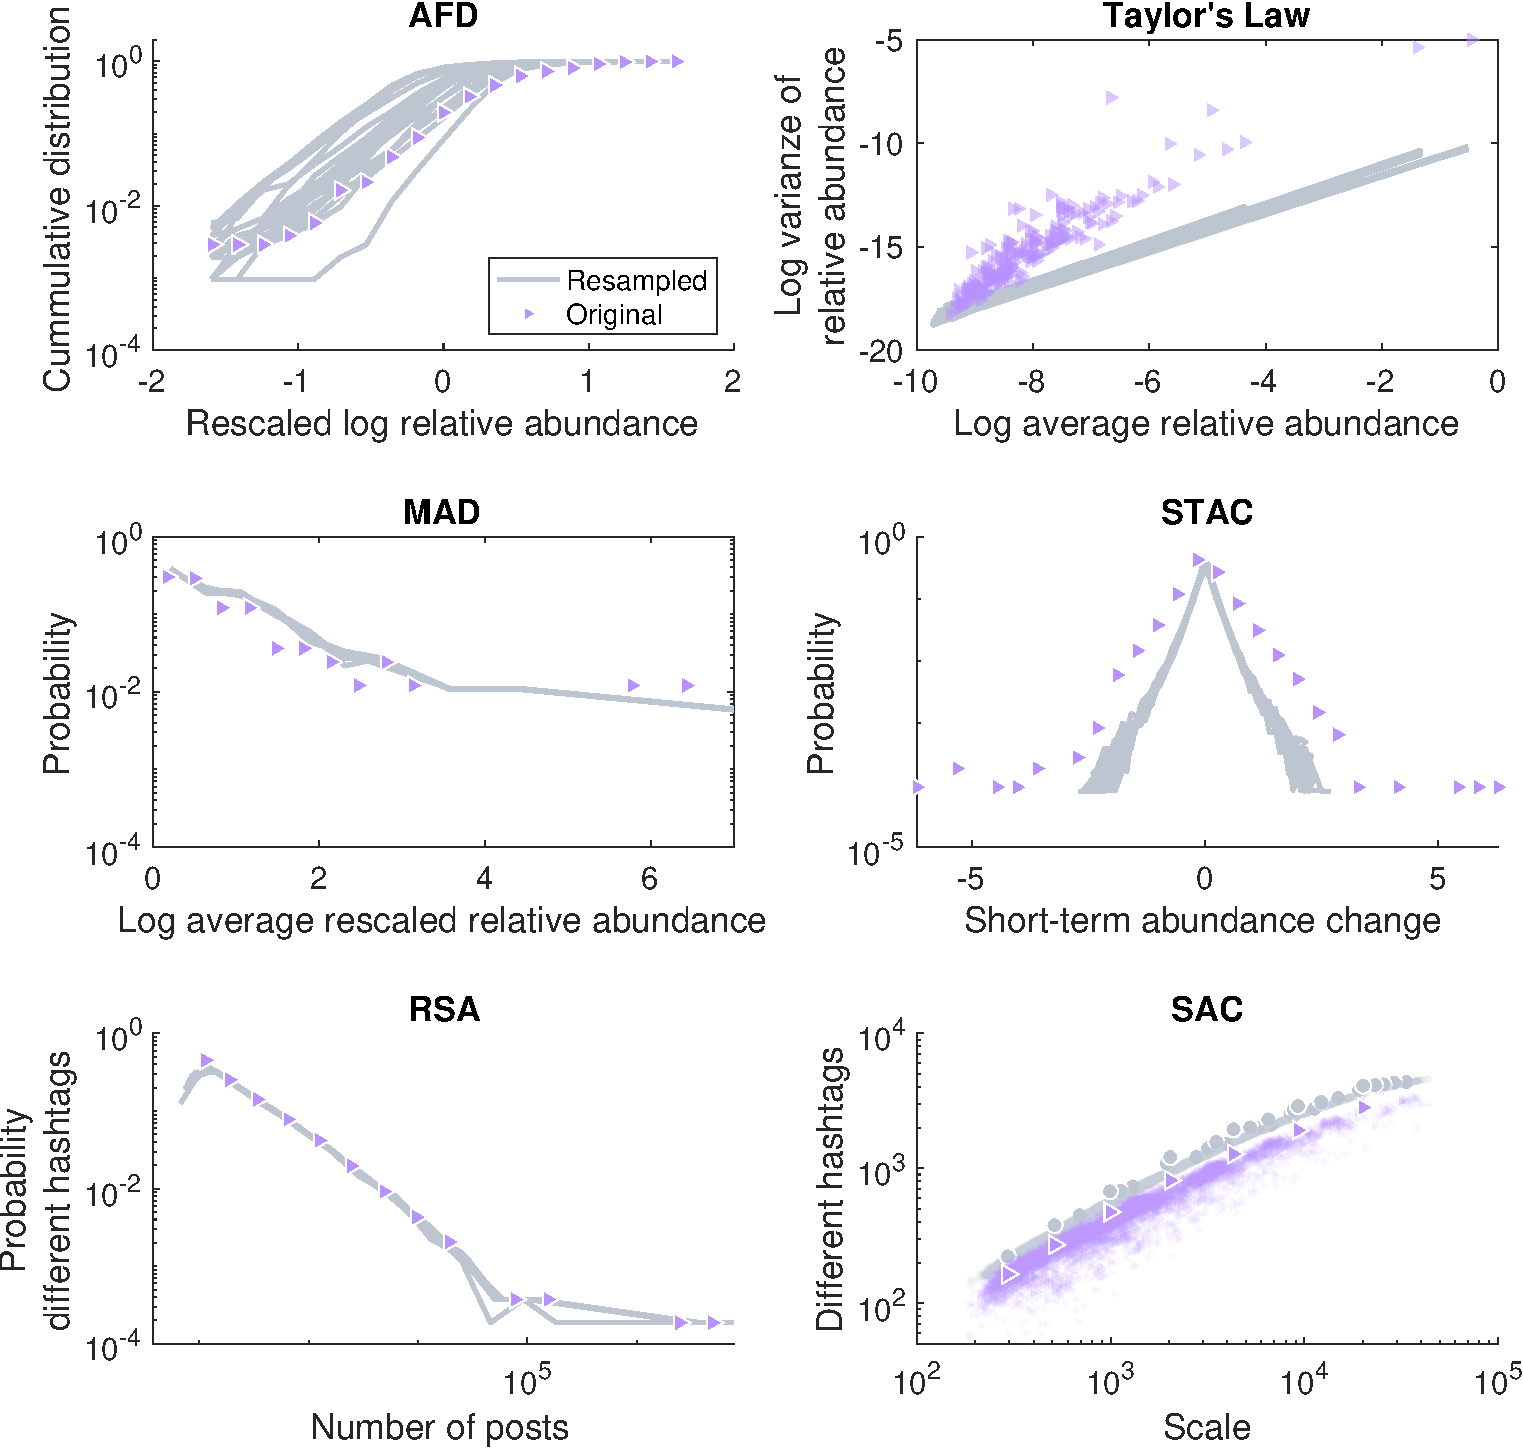
\includegraphics[width=\textwidth]{figures/chp4/Figure_Lego_Hurricane Sandy_25Apr_lines.pdf}
    \caption[Macropatterns with the multinomial random sampling model]{Macropatterns obtained by the multinomial random sampling model for the largest dataset (Hurricane Sandy) confronted with the original patterns, in colored dots. Each gray line corresponds to a resampling of the entire dataset.}
    \label{chp:4:fig:Lego}
\end{figure}

\section{Implications of finding macropatterns}
%%%%%%%%%%%%%%%%%%%%%%%%%%%%%%%%%%%%%%%%%%%%%%%%%%%%%%%%%%%%%%%%%%%%%%%%%%

In this Chapter, we have found that six patterns originally discovered in ecological communities also hold for online social networks. These patterns not only are present in a variety of different datasets, but also their functional forms and parameters are compatible with the ones found in ecology. These common characteristics can help to guide the search for the underlying processes that create the patterns in the first place. \\

To expose the drivers, we have begun by comparing the empirical patterns with the patterns generated by a null model fed just with the frequency of hashtags in the online social network \cite{lego}. We find that some patterns are incompatible with this simple process, invalidating the assumption that hashtags are used solely based on their frequency and pointing to the existence of general laws in these systems. In particular, three patterns are informative about the fundamental mechanisms behind the observed behavior: Taylor's law, which is the pattern that shows clearly a divergence from a multinomial process, followed by deviations of the AFD and STAC.\\

Even though the resolution and number of our datasets are limited, systematically finding the patterns for all of them makes our results nevertheless quite convincing. Each dataset has been generated by an intrinsically-imperfect sampling, but since we have included datasets with different sampling methods, the possible biases are reduced. Regarding the theoretical functional forms borrowed from ecology, they are based on assumptions that may be revisited to fully characterize the driving processes in online social networks. Moreover, given that the processes at the origin of our patterns --regardless of which they are-- consistently manifest themselves in the predicted forms, it is crucial to have a robust method for fitting the empirical data to the theoretical distributions \cite{leroi2020neutral}. Searching for these patterns --and other ecological patterns not covered here-- in more datasets and fitting them with alternative methods can give more hints about how online social networks operate at the macroscopic level. \\

The proposed ecological-social bridge is strengthened by finding these common patterns, which also opens the door to benefit from the existing body of theory developed in the study of macroecological patterns. Specifically, macropatterns have had important predictive power in ecology \cite{brown1995macroecology} that can be put to work for social systems \cite{tovo2021upscaling}. If we have characterized a set of patterns for OSNs, the presence of exogenous factors that threaten their health can be uncovered by looking at any deviation from the natural form of these patterns. With our analyses, we have found that Taylor's law, AFD, and STAC are sensitive to the underlying processes, making them promising candidates for detecting external interference in the usual dynamics of online social networks.